%------------------------------------------------------------------------------
%	Setup
%------------------------------------------------------------------------------
\documentclass[journal, twocolumn]{IEEEtran}


\usepackage{graphicx}
\usepackage[breaklinks=true]{hyperref}
\usepackage{amsmath}
\usepackage{multirow}
\usepackage{amssymb}

\usepackage{caption}
\usepackage{subcaption}
\captionsetup{font=footnotesize}

\usepackage{textcase}
\usepackage[tablename=TABLE]{caption}
\DeclareCaptionTextFormat{up}{\MakeTextUppercase{#1}}
\captionsetup[table]{
    labelsep=period,
    justification=centering,
    textformat=up,
}


% correct bad hyphenation here
\hyphenation{op-tical net-works semi-conduc-tor}


\begin{document}
%------------------------------------------------------------------------------
%	Title
%------------------------------------------------------------------------------
\title{An Automatic Face Attendance Checking System using Deep Facial Recognition Technique}


%------------------------------------------------------------------------------
%	Author
%------------------------------------------------------------------------------
\author{Thuy Nguyen-Chinh,
		Thien Do-Tieu,
		Phuong Le-Van-Hoang,
		Sy Nguyen-Tan,
		Qui Nguyen-Van,
		Phu Nguyen-Tan

\thanks{This work is our assignment in the course of "Artificial Intelligence in Control Engineering" Sep-Dec 2018, guided by Dr. Pham Viet Cuong (email: pvcuong@hcmut.edu.vn), Faculty of Electrical and Electronics Engineering, HoChiMinh city University of Technology.}
\thanks{Authors are senior of the Faculty of Electrical and Electronics Engineering, HoChiMinh city University of Technology (e-mail: \{thuy.ng.ch, dotieuthien9997, hpcqt97, tansyab1, nvqui97, tanphu97.nguyen \}@gmail.com).}
\thanks{The software is open source and can be found in \url{https://github.com/AntiAegis/Face-Attendance-System}.}
}


\maketitle


%------------------------------------------------------------------------------
%	Abstract
%------------------------------------------------------------------------------
\begin{abstract}
Nowadays, as computers are powerful enough for implementing complex algorithms, there are numerous applications that people utilize computers to run. In which, facial recognition is one of the most active fields of applications. In fact, computers can not only automatically identify who a person is, but also operate 24/7, which human beings cannot endure. This leads to the replacement of people by computers in some repetitive and real-time applications.

In this work, we apply the facial recognition into an attendance checking system that uses faces of registered people to check their attendance. This system has a GUI which allows easy user-to-system interaction. The core of the system is a deep facial recognition technique, which has four stages (e.g., removing motion-blur frames, detecting faces, removing non-frontal-view faces, and recognizing). Particularly, in the recognition phase, we consider this stage as an open-set facial recognition problem, so the system is able to detect people who have not registered in the database before. Also, we boost the performance of the system by utilizing hardware resources of users' computers. Although the system is designed to run with a low-resolution webcam, its performance is reasonably accurate on our private dataset.
\end{abstract}


\begin{IEEEkeywords}
Face Attendance Checking, Facial Recognition, Deep Learning
\end{IEEEkeywords}


\IEEEpeerreviewmaketitle


%------------------------------------------------------------------------------
%	Introduction
%------------------------------------------------------------------------------
\section{Introduction}
\label{introduction}
\textbf{This section is of Thien.}

Introduce about a framework of face recognition system, including face detection, landmark detection, face recognition.

\subsection{Face detection}

\subsection{Landmark detection}

\subsection{Face recognition}


%------------------------------------------------------------------------------
%	Proposed system
%------------------------------------------------------------------------------
\medskip
\section{Proposed system}
\label{proposed-system}

In this paper, we apply deep facial recognition techniques into the problem of face attendance checking. A system is built in order to manage appearances of students in a class. As normally, the system is organized as a pipeline of typical stages, namely face detection, landmark detection, and face recognition. However, to ensure input frames for underlying algorithms are high quality, we append an early filter that are able to discard blur frames, which are caught by motions of people in front of a standard webcam. Besides, we take a more step by adapting the landmark detection to verify whether a face is in frontal view of the camera so that the result of face recognition is more accurate. Also, to leverage the ease in use, the design a friendly graphic user interface (GUI) so that people who want to use the system to manage (teachers) or check (students) attendance can interact with the application without any specific knowledge. To make the system more robust, we carefully analyze the distribution outlier of features representing for registered accounts. Therefore, the algorithm has ability to detect people who have not registered in the application before, which is equivalent to the open-set problem in face recognition. Figure \ref{fig:system} reveals our proposed system.

Our work is organized as follows. In the section \ref{implementation}, stages of the proposed system are described clearly, including motion-blur detection, face detection, frontal-view detection, and face recognition. Then, section \ref{experimental-result} is for reporting some experimental results.


%------------------------------------------------------------------------------
%	Implementation
%------------------------------------------------------------------------------
\medskip
\section{Implementation}
\label{implementation}

\subsection{Motion-blur detection}
\label{motion-blur-detection}
\textbf{This section is of Phu.}

\subsection{Face detection}
\label{face-detection}
\textbf{This section is of Qui.}

\subsection{Frontal-view detection}
\label{frontal-view-detection}
\textbf{This section is of Qui.}

\subsection{Face recognition}
\label{face-recognition}
\textbf{This section is of Thien.}

\subsection{Graphic User Interface}
\label{gui}
\textbf{This section is of Sy.}


%----------------------------Attendance management-----------------------------
\subsection{Attendance management}
\label{attendance-management}
\textbf{This section is of Phuong.}

This is the final phase of Face Attendance Checking System.
It was designated to mark the presence of one resulted from
our algorithm in a file of excel format, namely xlsx extension.
To be used by the system, the excel file must meet
a stringent format made up of essential contents and be
generated by the GUI. 

Figure \ref{fig:form-new} depicts a new standard empty
excel table generated by our GUI. After obtaining a new file, we should fill in the table with the desired data (Figure \ref{fig:form-data}). The most special things in this table are column ID and Total. 
ID is considered a primary key because the algorithm will mark the presence of a specific person via his ID. 
To help the host in easy attendance management, we designed the column Total with a view to showing the number of absences in all.

Figure \ref{fig:form-checked} depicts an excel file's content after a checking progress finished. 
The GUI will automatically insert the only one new day column between Group and Total ones and in the tail of previous checked day. 
Letter 1 will be marked as presence in a cell of this column accordant to an ID. 
After attendance checking process is completed, the Total column will display the number of absences of previous days and the current one. Smartly can it display as we specially assigned a size-dynamic sum function to each cell of this column.


\begin{figure}
    \centering
    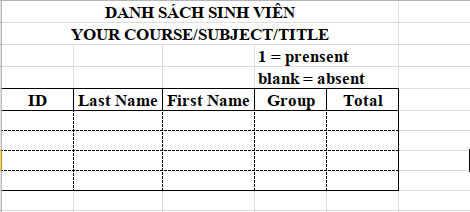
\includegraphics[width=0.8\linewidth]{img/form-new.png}
	\caption{New standard excel form}\label{fig:form-new}
\end{figure}

\begin{figure}
    \centering
    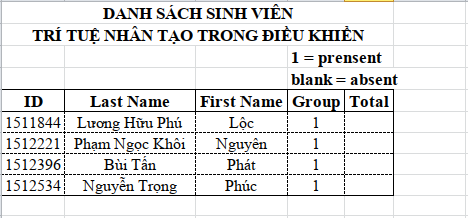
\includegraphics[width=0.8\linewidth]{img/form-data.png}
	\caption{Excel form contain pre-inputed data}\label{fig:form-data}
\end{figure}

\begin{figure}
    \centering
    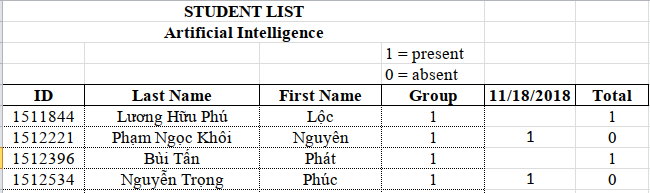
\includegraphics[width=0.8\linewidth]{img/form-checked.png}
	\caption{Form is under checking}\label{fig:form-checked}
\end{figure}


%------------------------------------------------------------------------------
%	Result
%------------------------------------------------------------------------------
\medskip
\section{Experimental result}
\label{experimental-result}
\textbf{This section is of Thien.}


%------------------------------------------------------------------------------
%	Conclusion
%------------------------------------------------------------------------------
\medskip
\section{Conclusion}
\label{conclusion}

In this work, we applied the deep facial recognition techniques to solve the problem of face attendance checking. The system has a pipeline with four stages (e.g., motion-blur detection, face detection, landmark detection, and face recognition). Besides, the system is also integrated a friendly GUI, which allows users both teachers and students interact with it in an easy way. On our private dataset, the application perform accurate despite of the low-resolution webcam of typical laptops. This demonstrates that our underlying algorithm is effective to deal with this poor-quality input problem.

In the future, we will target to widen our dataset so that the dataset will be asymptotic to real applications. In addition, more algorithms will be considered to improve the ability of the algorithm to discriminate feature distributions of output classes.


%------------------------------------------------------------------------------
%	Acknowledgment
%------------------------------------------------------------------------------
\section*{Acknowledgment}

The authors would like to thank Dr. Pham Viet Cuong for providing documents as well as chance for us to do this work. Also, the authors would like to thank ...


%------------------------------------------------------------------------------
% References
%------------------------------------------------------------------------------
\begin{thebibliography}{9}
%% Copy-Move-------------------------------------------------------------------
%%%% Key-point-based
\bibitem{ref:keypoint-1}
X. Pan and S. Lyu,
\textit{``Region duplication detection using image feature matching"},
IEEE Transactions on Information Forensics and Security,
vol. 5, no.4, ISSN: 1556-6013, pp. 857-867, 2010.
	
\bibitem{ref:keypoint-2}
I. Amerini, L. Ballan, R. Caldelli, A. Del Bimbo and G.Serra,
\textit{``A sift-based forensic method for copy–move attack detection and transformation recovery"},
IEEE Transactions on Information Forensics and Security,
vol. 6, no. 3, ISSN: 1556-6013, pp. 1099-1110, 2011.

\bibitem{ref:keypoint-3}
P. Kakar, N. Sudha,
\textit{``Exposing postprocessed copy-paste forgeries through transform-invariant feature"},
IEEE Transactions on Information Forensics and Security,
vol. 7, no. 3, ISSN: 1556-6013, pp. 1018-1028, June 2012.

%%%% Block-based
\bibitem{ref:block-1}
S.-J. Ryu, M.-J. Lee and H.-K. Lee,
\textit{``Detection of copy-rotate-move forgery using Zernike moments"},
Information Hiding Conference, Lecture Notes in Computer Science, vol. 6387, Springer,
Heidelberg-Berlin, 2010, ISBN: 978-3-642-16434-7.

\bibitem{ref:block-2}
H.-J. Lin, C.-W. Wang and Y.-T. Kao,
\textit{``Fast copy-move forgery detection"},
WSEAS Transactions on Signal Processing,
vol. 5, no. 5, ISSN: 0031-3203, pp. 188-1975, 2009.

\bibitem{ref:block-3}
V. Christlein, C. Riess, J. Jordan and E. Angelopoulou,
\textit{``An evaluation of popular copy-move forgery detection approaches"},
IEEE Transactions on Information Forensics and Security,
vol. 7, no. 6, ISSN: 1556-6013, pp. 1841-1854, 2012.

\bibitem{ref:block-4}
T. L.-Tien, T. H.-Kha, L. P.-C.-Hoan, A. T.-Hong, N. Dey, M. Luong,
\textit{``Combined Zernike Moment and Multiscale Analysis for Tamper Detection in Digital Images"},
Informatica (An International Journal of Computing and Informatics),
vol.41, no.1, ISSN: 0350-5596, March 2017.


%% JPEG format-----------------------------------------------------------------
\bibitem{ref:jpeg-dct-1}
Z. Lin, J. He, X. Tang, K. Tang,
\textit{``Fast, automatic and fine-grained tampered JPEG image detection via DCT coefficient analysis"},
Pattern Recognition, vol. 42, no. 11, ISSN: 0031-3203, pp. 2492-2501, January 2009.

\bibitem{ref:jpeg-dct-2}
W. Wang, J. Dong, T. Tan,
\textit{``Exploring DCT coefficient quantization effects for local tampering detection"},
IEEE Transactions on Information Forensics and Security,
vol. 9, no. 10, ISSN: 1556-6013, pp. 1653-1666, October 2014.

\bibitem{ref:jpeg-periodicity}
L. Chen, T. Hsu,
\textit{``Detecting recompression of JPEG images via periodicity analysis of compression artifacts for tampering detection"},
IEEE Transactions on Information Forensics and Security,
vol. 6, no. 2, ISSN: 1556-6013, pp. 396-406, June 2011.

\bibitem{ref:jpeg-improved}
L. Thing, Y. Chen, C. Cheh,
\textit{``An improved double compression detection method for JPEG image forensics"},
In IEEE International Symposium on Multimedia,
pages 290-297, December 2012, ISBN: 978-1-4673-4370-1.

\bibitem{ref:jpeg-ghosts}
F. Zach, C. Riess, and E. Angelopoulou,
\textit{``Automated image forgery detection through classification of JPEG ghosts"},
Pattern Recognition, 7476, pp. 185-194, January 2012.

\bibitem{ref:jpeg-block-grained}
T. Bianchi, A. Piva,
\textit{``Image forgery localization via block-grained analysis of JPEG artifacts"},
IEEE Transactions on Information Forensics and Security,
vol. 7, no. 3, ISSN: 1556-6013, pp. 1003-1017, June 2012.

\bibitem{ref:jpeg-inpainting}
C. Chang, C. Yu, C. Chang,
\textit{``A forgery detection algorithm for exemplar-based inpainting images using multi-region relation"},
Journal Image and Vision Computing,
vol. 31, no. 1, ISSN: 0262-8856, pp. 57-71, MA-USA, 2013.


%% Deep Learning approach------------------------------------------------------
\bibitem{ref:cnn-median}
J. Chen, X. Kang, Y. Liu and Z. J. Wang,
\textit{``Median Filtering Forensics Based on Convolutional Neural Networks"},
IEEE Signal Processing Letters,
vol. 22, no. 11, ISSN: 1070-9908, pp. 1849-1853, November 2015.

\bibitem{ref:cnn-universal}
B. Bayar, M. C. Stamm,
\textit{``A Deep Learning Approach to Universal Image Manipulation Detection Using a New Convolutional Layer"},
Proceedings of the 4th ACM Workshop on Information Hiding and Multimedia Security,
pp. 5-10, New York-USA, 2016, ISBN: 978-1-4503-4290-2.

\bibitem{ref:cnn-srm}
Rao Yuan, Ni Jiangqun,
\textit{``A deep learning approach to detection of splicing and copy-move forgeries in images"},
IEEE International Workshop on Information Forensics and Security (WIFS),
Abu Dhabi-United Arab Emirates, 2016, ISBN: 978-1-5090-1139-1.

\bibitem{ref:cnn-alex}
J.Ouyang, Y.Liu, M.Liao,
\textit{``Copy-Move Forgery Detection Based on Deep Learning"},
10th International Congress on Image and Signal Processing, BioMedical Engineering and Informatics,
Shanghai-China, 2017, ISBN: 978-1-5386-1938-4.

\bibitem{ref:dae}
Y. Zhang, J. Goh, L. Win, V. Thing,
\textit{``Image Region Forgery Detection: A Deep Learning Approach"},
Proceedings of the Singapore Cyber-Security Conference, Singapore, 2016, ISBN: 978-1-61499-616-3.


%% Database--------------------------------------------------------------------
\bibitem{ref:casia}
J. Dong and W. Wang,
\textit{``Casia tampering detection dataset"}, 2011.


%% Machine Learning------------------------------------------------------------
\bibitem{ref:alex-net}
A. Krizhevsky, I. Sutskever, G. Hinton,
\textit{``Imagenet classification with deep convolutional neural networks"},
NIPS'12 Proceedings of the 25th International Conference on Neural Information Processing Systems,
vol. 1, pp. 1097-1105, Nevada-USA, 2012, DOI: 10.1145/3065386.

\bibitem{ref:dropout}
N. Srivastava, 	G. Hinton, A. Krizhevsky, I. Sutskever, R. Salakhutdinov,
\textit{``Dropout: a simple way to prevent neural networks from overfitting"},
The Journal of Machine Learning Research,
vol. 15, no. 1, ISSN 1533-7928, pp. 1929-1958, January 2014.

\bibitem{ref:xavier}
Xavier Glorot, Yoshua Bengio,
\textit{``Understanding the difficulty of training deep feedforward neural networks"},
Proceedings of the 13rd International Conference on Artificial Intelligence and Statistics,
PMLR 9, pp. 249-256, Sardinia-Italy, \url{http://proceedings.mlr.press/v9/glorot10a/glorot10a.pdf}, 2010.

\bibitem{ref:relu}
V. Nair, E. Hinton,
\textit{``Rectified Linear Units Improve Restricted Boltzmann Machines"},
Proceedings of the 27th International Conference on Machine Learning,
pp. 807-814, Haifa-Israel, 2010, ISBN: 978-1-60558-907-7.

\bibitem{ref:leaky-relu-1}
B. Xu, N. Wang, T. Chen, M. Li,
\textit{``Empirical Evaluation of Rectified Activations in Convolutional Network"},
\url{https://arxiv.org/abs/1505.00853v2}, 2015.

\bibitem{ref:leaky-relu-2}
K. He, X. Zhang, S. Ren, J. Sun
\textit{``Delving Deep into Rectifiers: Surpassing Human-Level Performance on ImageNet Classification"},
\url{https://arxiv.org/abs/1502.01852v1}, 2015.

\bibitem{ref:adam}
P. Kingma, J. Ba,
\textit{``Adam: A Method for Stochastic Optimization"},
3rd International Conference for Learning Representations, San Diego-USA,
\url{https://arxiv.org/abs/1412.6980}, 2015.


%% Comparison------------------------------------------------------------------
\bibitem{ref:goh}
J. Goh and V. L. L. Thing,
\textit{``A hybrid evolutionary algorithm for feature and ensemble selection in image tampering detection"},
International Journal of Electronic Security and Digital Forensics,
vol. 7, no. 1, ISSN: 1751-911X, pp. 76-104, March 2015.

\bibitem{ref:he}
Z. He, W. Lu, W. Sun, J. Huang,
\textit{``Digital image splicing detection based on Markov features in DCT and DWT domain"},
Pattern Recognition, vol. 45, no. 12, ISSN: 0031-3203, pp. 4292-4299, 2012.


%% Appendix--------------------------------------------------------------------
\bibitem{ref:prove-wavelet}
A. Cohen, T. Tiplica, and A. Kobi,
\textit{``Design of experiments and statistical process control using wavelets analysis"},
Control Engineering Practice,
vol. 49, ISSN: 0967-0661, pp. 129-183, April 2016.


\end{thebibliography}

\end{document}